\documentclass[10pt, aspectratio=169]{beamer}

% --- Theme and Customization ---
\usetheme[progressbar=frametitle]{metropolis}
\useoutertheme{miniframes}

% Force navigation dots in the headline
\setbeamertemplate{headline}{%
    \begin{beamercolorbox}[colsep=1.5pt]{upper separation line head}
    \end{beamercolorbox}
    \begin{beamercolorbox}{section in head/foot}
        \insertnavigation{\paperwidth}
    \end{beamercolorbox}%
}

% Color adjustments for visual appeal
\definecolor{DarkSteel}{RGB}{45, 55, 72}
\definecolor{AccentBlue}{RGB}{49, 130, 206}
\definecolor{AccentRed}{RGB}{197, 48, 48}
\definecolor{MutedGrey}{RGB}{160, 174, 192}
\setbeamercolor{frametitle}{bg=DarkSteel, fg=white}
\setbeamercolor{progress bar}{fg=AccentBlue, bg=gray!30}
\setbeamercolor{block title}{bg=DarkSteel!10, fg=DarkSteel}
\setbeamercolor{block body}{bg=DarkSteel!5, fg=black}
\setbeamercolor{section in head/foot}{bg=white, fg=DarkSteel}

\metroset{block=fill}

\usepackage[utf8]{inputenc}
\usepackage{booktabs}
\usepackage{tikz}
\usetikzlibrary{arrows.meta, decorations.pathreplacing, positioning}

% Figures live one directory up
\graphicspath{{../results/figures/}}

% --- Metadata ---
\title{Do LLMs Shape the Diffusion of New Software?}
\subtitle{Training Cutoffs and Adoption Dynamics in the Python Ecosystem}
\author{Roland Tuboly \\ \small MSc Social Data Science}
\date{TDK Presentation --- May 2026}

\begin{document}

\maketitle

% =========================================================
\section{Motivation}
% =========================================================

\begin{frame}{Why software diffusion, and why now?}
    \begin{columns}[T]
        \begin{column}{0.55\textwidth}
            \begin{block}{The measurable object}
                Software libraries are a clean unit of technological diffusion: released on a date, downloaded at a measurable rate, used in public code.
            \end{block}
            \begin{block}{Why it matters}
                \begin{itemize}
                    \item \textbf{Productivity vs.\ variety} --- Doshi \& Hauser (2024): individual gains can narrow collective variety.
                    \item \textbf{Knowledge frontier} --- Acemoglu (2024); Evans; Daniotti et al.\ on scientific search.
                    \item \textbf{Gatekeeping} --- Wachs on platforms steering adoption.
                \end{itemize}
            \end{block}
        \end{column}
        \begin{column}{0.42\textwidth}
            \begin{alertblock}{Research question}
                Do Python libraries released \emph{after} an LLM's training cutoff diffuse more slowly than otherwise-identical libraries released \emph{before} the cutoff?
            \end{alertblock}
        \end{column}
    \end{columns}
\end{frame}

% =========================================================
\section{Method}
% =========================================================

\begin{frame}{Method at a glance}
    \begin{columns}[T]
        \begin{column}{0.48\textwidth}
            \begin{block}{Option A --- Single-year RDD}
                Compare libraries released just before vs.\ just after Sept 2021, within a narrow bandwidth.
                \\[0.5em]
                \textbf{Problem:} the jump we see is a mix of the LLM effect \emph{and} raw calendar seasonality (September releases differ from August releases every year).
            \end{block}
        \end{column}
        \begin{column}{0.48\textwidth}
            \begin{exampleblock}{Option B --- Diff-in-RDD (ours)}
                Stack 2018--2020 placebo cohorts at the same calendar position. Subtract the placebo jump from the 2021 jump.
                \\[0.5em]
                \textbf{Payoff:} seasonality is differenced out; the residual is the LLM-specific treatment effect.
            \end{exampleblock}
        \end{column}
    \end{columns}
    \vfill
    \footnotesize \emph{Both estimators are reported. The Diff-in-RDD is our primary specification.}
\end{frame}

% =========================================================
\section{Data}
% =========================================================

\begin{frame}{Data and unit of analysis}
    \begin{columns}[T]
        \begin{column}{0.50\textwidth}
            \begin{block}{Sources}
                \begin{itemize}
                    \item \textbf{PyPI}: weekly downloads for every registered package.
                    \item \textbf{GitHub}: code-import counts (linked sample).
                \end{itemize}
            \end{block}
            \begin{block}{Panel}
                Library-week, from first release through January 2026.
            \end{block}
        \end{column}
        \begin{column}{0.46\textwidth}
            \begin{exampleblock}{Scale}
                \begin{itemize}
                    \item \textbf{527{,}361} PyPI packages.
                    \item \textbf{28{,}243} linked to GitHub.
                    \item \textbf{88{,}001} in Diff-in-RDD (Broad tier).
                    \item Cutoff: \textbf{September 2021} (GPT-3.5 / GPT-4 knowledge boundary).
                \end{itemize}
            \end{exampleblock}
        \end{column}
    \end{columns}
\end{frame}

% =========================================================
\section{Design}
% =========================================================

\begin{frame}{Design timeline}
    \centering
    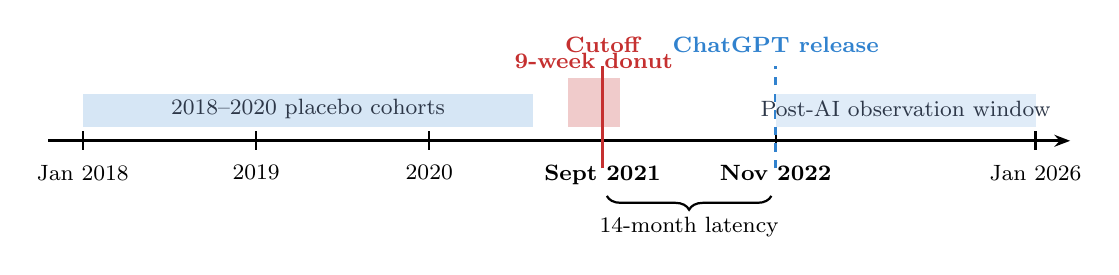
\begin{tikzpicture}[x=1.1cm, y=1cm, >={Stealth[length=2mm]}]
        % axis
        \draw[very thick, ->] (-0.4,0) -- (11.4,0);
        % major ticks + labels
        \foreach \x/\lbl in {0/Jan 2018, 2/2019, 4/2020, 6/\textbf{Sept 2021}, 8/\textbf{Nov 2022}, 11/Jan 2026} {
            \draw[thick] (\x,0.12) -- (\x,-0.12);
            \node[below=2pt, align=center, font=\footnotesize] at (\x,-0.12) {\lbl};
        }
        % placebo years band (shaded)
        \fill[AccentBlue!20] (0,0.18) rectangle (5.2,0.6);
        \node[font=\footnotesize, DarkSteel] at (2.6,0.4) {2018--2020 placebo cohorts};
        % donut
        \fill[AccentRed!25] (5.6,0.18) rectangle (6.2,0.8);
        \node[font=\footnotesize\bfseries, AccentRed, above] at (5.9,0.8) {9-week donut};
        % cutoff marker
        \draw[AccentRed, very thick] (6,-0.35) -- (6,0.95);
        \node[font=\footnotesize\bfseries, AccentRed, above] at (6,1.0) {Cutoff};
        % ChatGPT marker
        \draw[AccentBlue, very thick, dashed] (8,-0.35) -- (8,0.95);
        \node[font=\footnotesize\bfseries, AccentBlue, above] at (8,1.0) {ChatGPT release};
        % latency brace
        \draw[decorate, decoration={brace, amplitude=5pt, mirror}, thick] (6.05,-0.7) -- (7.95,-0.7);
        \node[font=\footnotesize, below] at (7,-0.85) {14-month latency};
        % post-AI observation window
        \fill[AccentBlue!15] (8,0.18) rectangle (11,0.6);
        \node[font=\footnotesize, DarkSteel] at (9.5,0.4) {Post-AI observation window};
    \end{tikzpicture}
    \vfill
    \footnotesize \emph{The September 2021 cutoff is an invisible property of training data; libraries released a week before or after look identical to a developer in 2021. No one could have anticipated ChatGPT, released 14 months later.}
\end{frame}

\begin{frame}{Identification}
    \begin{itemize}
        \item \textbf{As-if random assignment}: the exact week of release relative to an invisible training cutoff is exogenous to the library itself (McCrary density test: $p = 0.43$).
        \item \textbf{RDD specifics}: bandwidth $h = 13$ weeks; local-linear regression with triangular kernel; 9-week donut excludes the Aug--Sept 2021 window of ambiguous training inclusion.
        \item \textbf{Inference}: cluster-robust standard errors at the year-by-week level (${\sim}72$ clusters); bias-corrected CIs via \texttt{rdrobust}.
        \item \textbf{Diff-in-RDD}: the 2021 discontinuity minus the mean placebo discontinuity (2018--2020) isolates the LLM-specific effect from calendar seasonality.
    \end{itemize}
\end{frame}

\begin{frame}{Validity diagnostics}
    \begin{itemize}
        \item \textbf{No manipulation}: McCrary density smooth across the cutoff ($p = 0.43$) --- developers cannot time their release to an unannounced boundary.
        \item \textbf{Covariate balance, pre-AI}: post-cutoff libraries actually start \emph{ahead} on pre-ChatGPT downloads (a seasonal headwind for our hypothesis) --- so the post-AI suppression is a \textbf{conservative} estimate.
        \item \textbf{Placebo years}: 2018--2020 cohorts show no discontinuity at the same calendar position, ruling out seasonality as the driver.
    \end{itemize}
\end{frame}

% =========================================================
\section{Results}
% =========================================================

\begin{frame}{Headline}
    \centering
    \vspace{0.3em}
    {\color{DarkSteel}\fontsize{22}{26}\selectfont Post-cutoff libraries have}\\[0.5em]
    {\color{AccentRed}\fontsize{96}{110}\selectfont\bfseries $+430\%$}\\[0.6em]
    {\color{DarkSteel}\fontsize{22}{26}\selectfont fewer weekly downloads by January 2026.}\\[1.2em]
    \begin{minipage}{0.8\textwidth}
        \centering
        \footnotesize
        Ratio of pre-cutoff to post-cutoff downloads, Jan 2026 vs.\ matched post-ChatGPT window. Diff-in-RDD confirms the gap: $p = 0.001$ (Broad tier), $p = 0.002$ (Successful tier), baseline-adjusted, cluster-robust SE.
    \end{minipage}
\end{frame}

\begin{frame}{Activation dynamics}
    \begin{columns}[T]
        \begin{column}{0.40\textwidth}
            \begin{itemize}
                \item \textbf{Dormant}: gap flat at ${\sim}28\%$ seasonal baseline before Nov 2022.
                \item \textbf{Activation}: discontinuity emerges only after ChatGPT's mass adoption.
                \item \textbf{Trajectory}: $+136\%$ at 12 months, $+287\%$ at 24 months, $+430\%$ by Jan 2026.
                \item Shaded band: $95\%$ bootstrap CI.
            \end{itemize}
        \end{column}
        \begin{column}{0.58\textwidth}
            \begin{figure}
                \centering
                \setlength{\fboxrule}{0.4pt}
                \setlength{\fboxsep}{0pt}
                \fbox{
\includegraphics[width=\linewidth]{normalized_diffusion_gap_pypi.png}}
            \end{figure}
        \end{column}
    \end{columns}
\end{frame}

\begin{frame}{Mechanism: GitHub imports}
    \begin{columns}[T]
        \begin{column}{0.48\textwidth}
            \begin{block}{Directional evidence}
                \begin{itemize}
                    \item Matched subsample, $N = 6{,}582$ in Diff-in-RDD.
                    \item All-time imports: $+2.12$ log-point jump (baseline-adjusted, $p = 0.022$) --- post-cutoff libraries accumulate \emph{more} GitHub imports, \textbf{opposite} sign to PyPI.
                \end{itemize}
            \end{block}
        \end{column}
        \begin{column}{0.48\textwidth}
            \begin{block}{Interpretation}
                \begin{itemize}
                    \item PyPI downloads are a \textbf{flow}; GitHub imports are a \textbf{stock} of existing code.
                    \item New libraries displace old ones in flow, but existing repos keep their old imports.
                    \item Consistent with LLM steering: the LLM pushes the \emph{first try}, not every line of legacy code.
                \end{itemize}
            \end{block}
        \end{column}
    \end{columns}
\end{frame}

\begin{frame}{Moderation \& scope}
    \begin{itemize}
        \item \textbf{AI-exposure heterogeneity}: directional but non-significant ($p = 0.18$) --- suggests a broad, systemic effect rather than a subset-specific channel.
        \item \textbf{Ecosystem}: Python only. Rust, JS, R may show different magnitudes.
        \item \textbf{One cutoff}: effects estimated around September 2021; newer-model cutoffs would require separate estimation.
        \item \textbf{SUTVA}: gap reflects direct suppression plus substitution toward established tools --- both are part of the LLM effect.
    \end{itemize}
\end{frame}

% =========================================================
\section{Discussion}
% =========================================================

\begin{frame}{Implications}
    \begin{block}{The Knowledge Wall}
        Training-data cutoffs act as a functional barrier for newly released software tools.
    \end{block}
    \begin{itemize}
        \item \textbf{Durable advantage}: tools embedded in LLM weights gain persistent visibility.
        \item \textbf{Spillovers}: same logic plausibly applies to research papers, blog posts, documentation.
        \item \textbf{Policy}: raises questions about how AI systems update their internal knowledge and what the costs are of being ``outside the wall''.
    \end{itemize}
\end{frame}

\begin{frame}{Limitations}
    \begin{itemize}
        \item We observe outcomes (downloads, imports), not LLM usage directly.
        \item AI systems are evolving --- web search and retrieval may erode the wall over time.
        \item One language, one cutoff, one year of treatment --- external validity is local.
        \item Running variable is release date; metadata errors could attenuate estimates.
    \end{itemize}
\end{frame}

% =========================================================
\section{Conclusion}
% =========================================================

\begin{frame}{Conclusion}
    \begin{alertblock}{}
        \centering \Large
        A $+430\%$ diffusion gap by January 2026, activated only after ChatGPT,
        \\
        with no placebo discontinuities --- a clean quasi-experiment
        \\
        for \emph{collective narrowing} in the age of LLMs.
    \end{alertblock}
    \vfill
    \begin{itemize}
        \item LLMs steer adoption toward tools already in training data.
        \item Libraries released post-cutoff face persistent disadvantages.
        \item The Knowledge Wall is real, measurable, and widening.
    \end{itemize}
\end{frame}

\begin{frame}[standout]{}
    \centering
    {\Huge Thank you.}\\[1em]
    {\Large Questions?}\\[2em]
    \begin{tikzpicture}[x=0.75cm, y=0.5cm, >={Stealth[length=1.5mm]}]
        \draw[thick, white, ->] (-0.2,0) -- (11.2,0);
        \foreach \x/\lbl in {0/2018, 6/{Sept '21}, 8/{Nov '22}, 11/{Jan '26}} {
            \draw[thick, white] (\x,0.08) -- (\x,-0.08);
            \node[below=1pt, font=\scriptsize, white] at (\x,-0.08) {\lbl};
        }
        \draw[white, very thick] (6,-0.2) -- (6,0.4);
        \draw[white, very thick, dashed] (8,-0.2) -- (8,0.4);
        \node[font=\scriptsize, white, above] at (6,0.4) {cutoff};
        \node[font=\scriptsize, white, above] at (8,0.4) {ChatGPT};
    \end{tikzpicture}
    \\[1em]
    {\Large \textbf{+430\%} diffusion gap by Jan 2026.}
\end{frame}

% =========================================================
\appendix
\section*{Appendix}
% =========================================================

\begin{frame}{A1. Summary statistics}
    \centering
    \footnotesize
    \begin{tabular}{lrrr}
        \toprule
        Horizon & Pre-cutoff mean & Post-cutoff mean & $\Delta\%$ \\
        \midrule
        ChatGPT + 6 months  & 1{,}467 & 630   & $+133\%$ \\
        ChatGPT + 12 months & 2{,}559 & 1{,}085 & $+136\%$ \\
        ChatGPT + 24 months & 8{,}218 & 2{,}124 & $+287\%$ \\
        January 2026        & 18{,}085 & 3{,}410 & $\mathbf{+430\%}$ \\
        \midrule
        Post-ChatGPT average & 6{,}538 & 1{,}703 & $+284\%$ \\
        \bottomrule
    \end{tabular}
    \vspace{0.8em}
    \begin{itemize}
        \footnotesize
        \item Weekly PyPI downloads, mean across libraries in each cohort.
        \item Pre-cutoff: libraries released Jan--Aug 2021. Post-cutoff: Oct 2021--.
    \end{itemize}
\end{frame}

\begin{frame}{A2. Diff-in-RDD estimates (PyPI)}
    \centering
    \footnotesize
    \begin{tabular}{llrrrr}
        \toprule
        Panel & Tier & Excess jump & Cluster SE & $p$ & $N$ \\
        \midrule
        Pre-ChatGPT baseline     & Successful & $-3.72$ & 1.67 & 0.026 & 75{,}313 \\
        \midrule
        Post-ChatGPT, adjusted   & Broad      & $-7.29$ & 2.20 & \textbf{0.001} & 88{,}001 \\
        Post-ChatGPT, adjusted   & Successful & $-7.29$ & 2.39 & \textbf{0.002} & 75{,}313 \\
        Post-ChatGPT, adjusted   & Superstar  & $-0.25$ & 0.35 & 0.473 & 57{,}931 \\
        \midrule
        Post-ChatGPT, unadjusted & Broad      & $-9.14$ & 4.42 & 0.039 & 88{,}001 \\
        Post-ChatGPT, unadjusted & Successful & $-12.79$ & 4.83 & 0.008 & 75{,}313 \\
        \bottomrule
    \end{tabular}
    \vspace{0.8em}
    \begin{itemize}
        \footnotesize
        \item Log-scale estimates: the discontinuity in log($1 + $downloads) at the cutoff, differenced against 2018--2020 placebos.
        \item Baseline adjustment: ANCOVA on log pre-ChatGPT downloads; absorbs level differences.
    \end{itemize}
\end{frame}

\begin{frame}{A3. Bandwidth sensitivity}
    \centering
    
\includegraphics[width=0.82\linewidth]{sensitivity_diff_in_rdd_bandwidth.png}\\
    \footnotesize \emph{Point estimate and 95\% CI across bandwidth choices $h \in \{10, 13, 18, 26, 39, 52\}$ weeks. Sign and significance stable.}
\end{frame}

\begin{frame}{A4. Density test and placebo years}
    \begin{columns}[T]
        \begin{column}{0.48\textwidth}
            \centering
            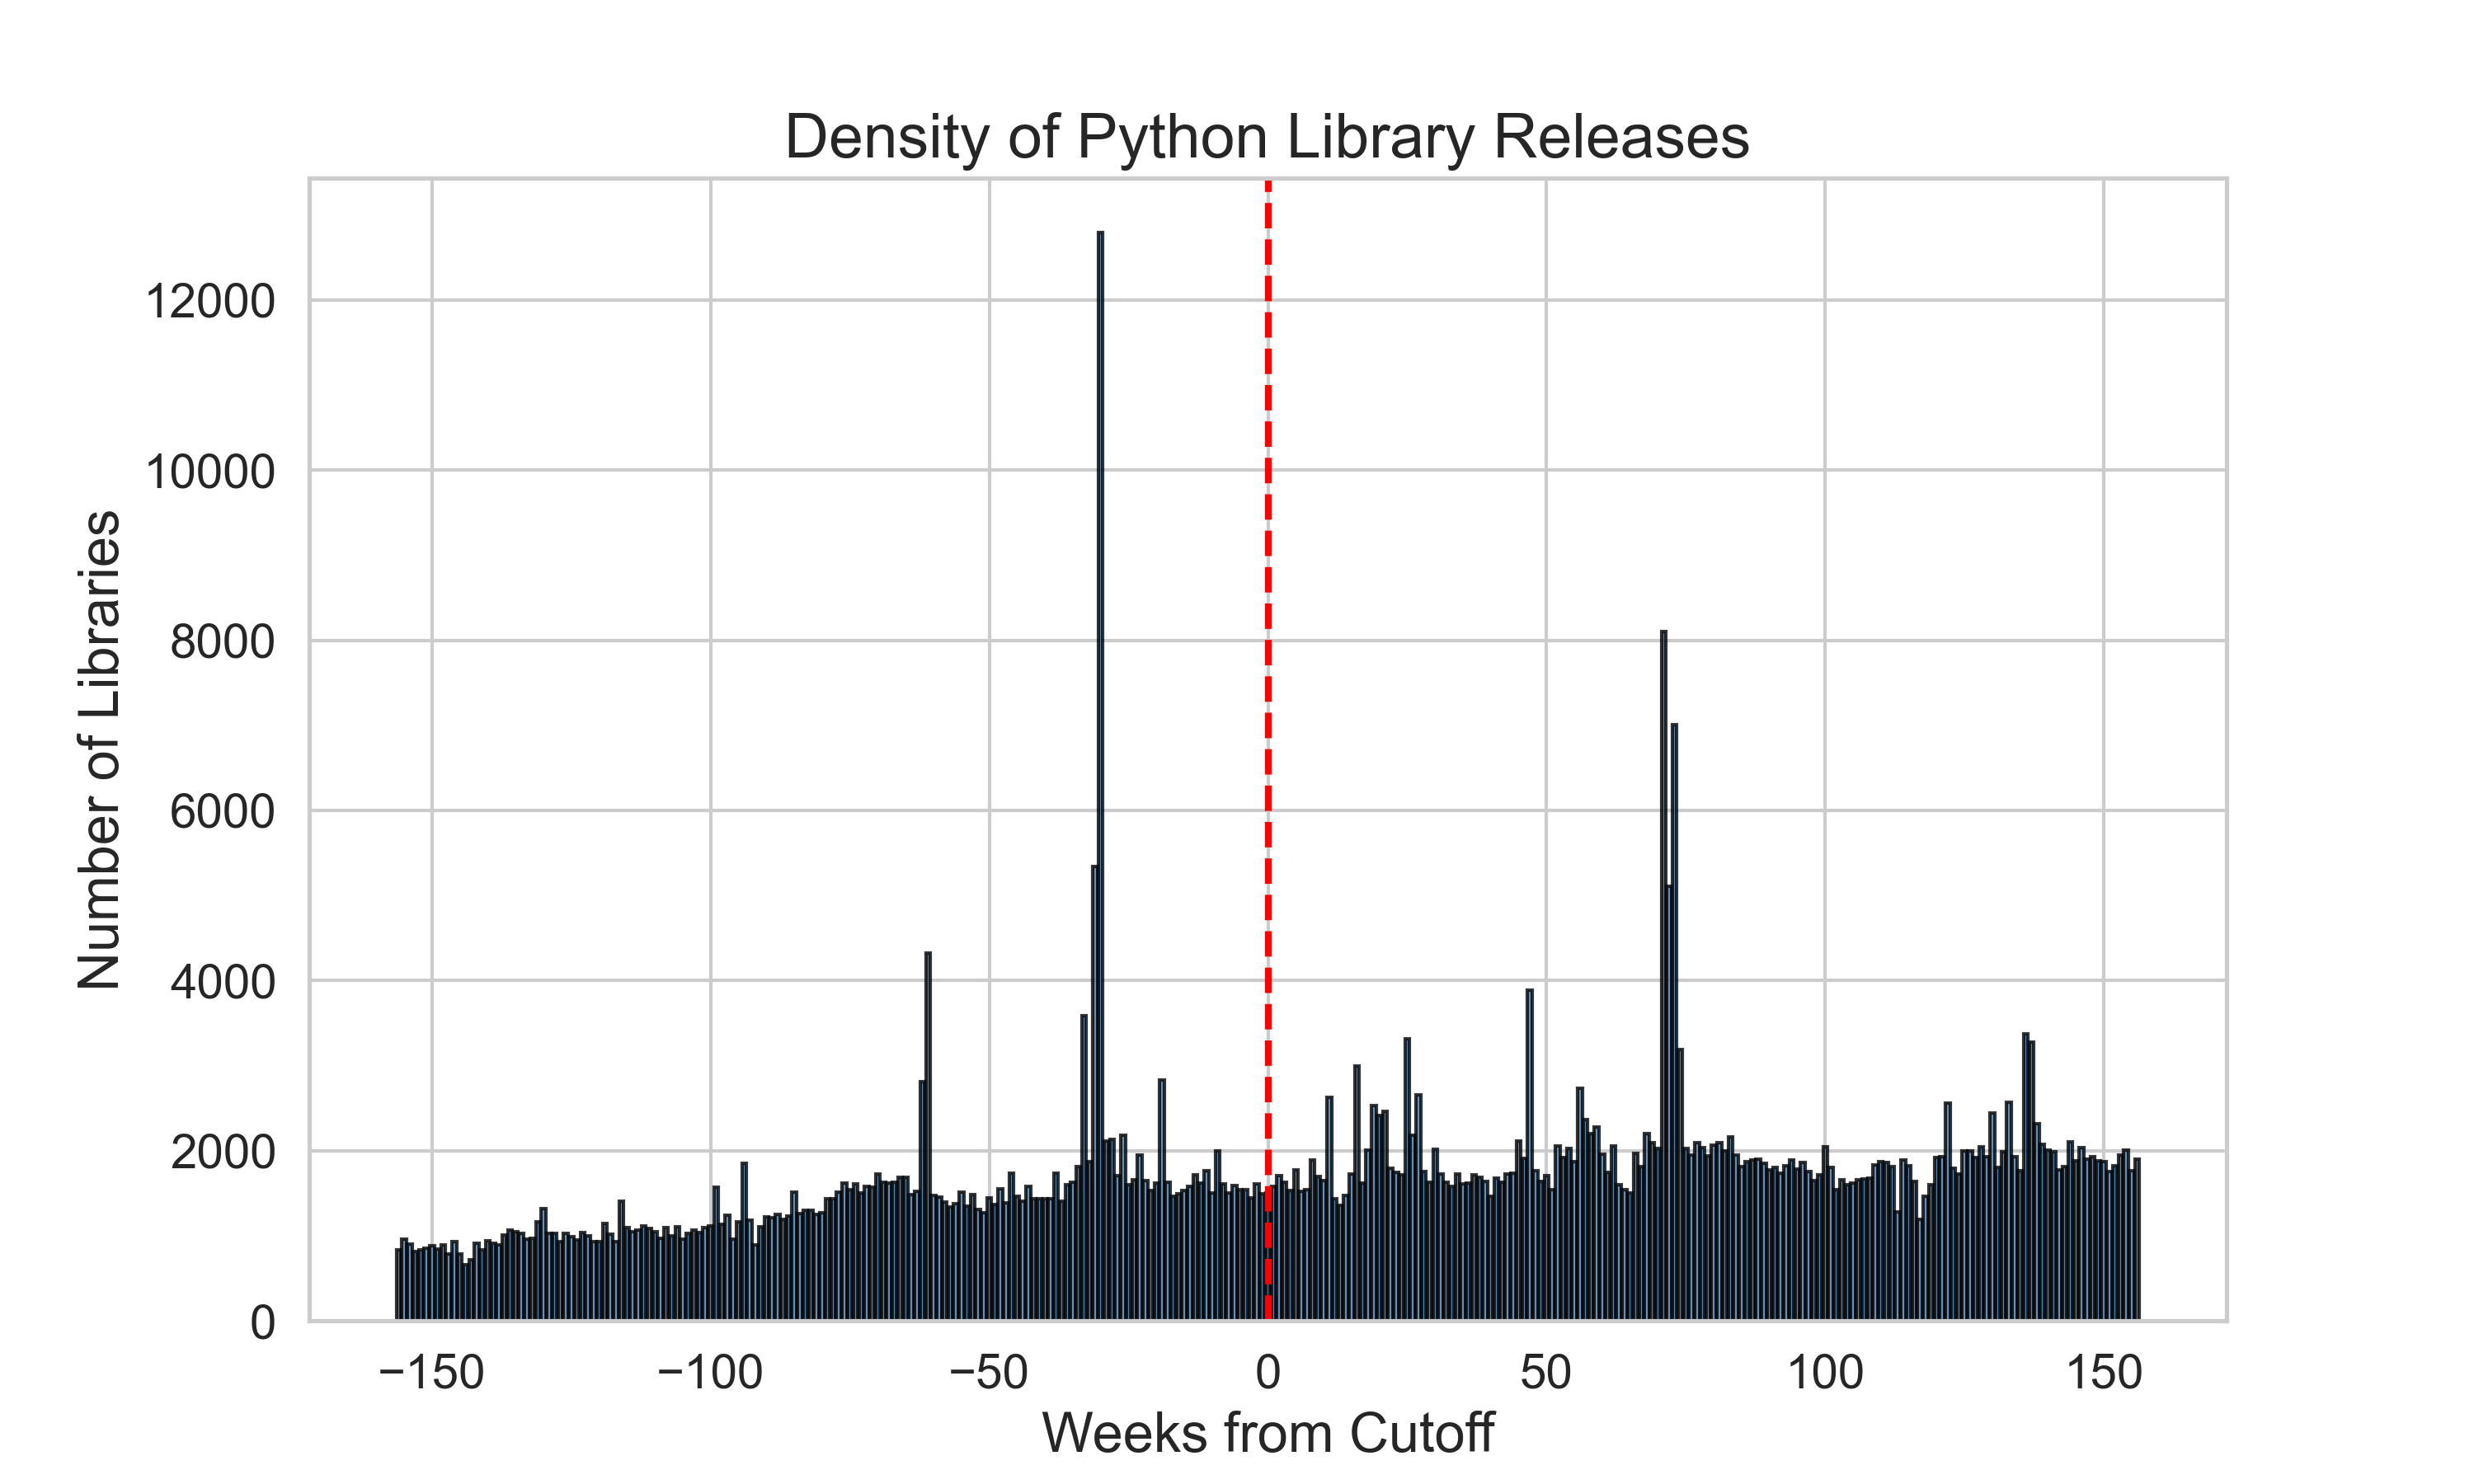
\includegraphics[width=\linewidth]{density_dist_to_cutoff.png}\\
            \footnotesize McCrary density, $p = 0.43$.
        \end{column}
        \begin{column}{0.48\textwidth}
            \centering
            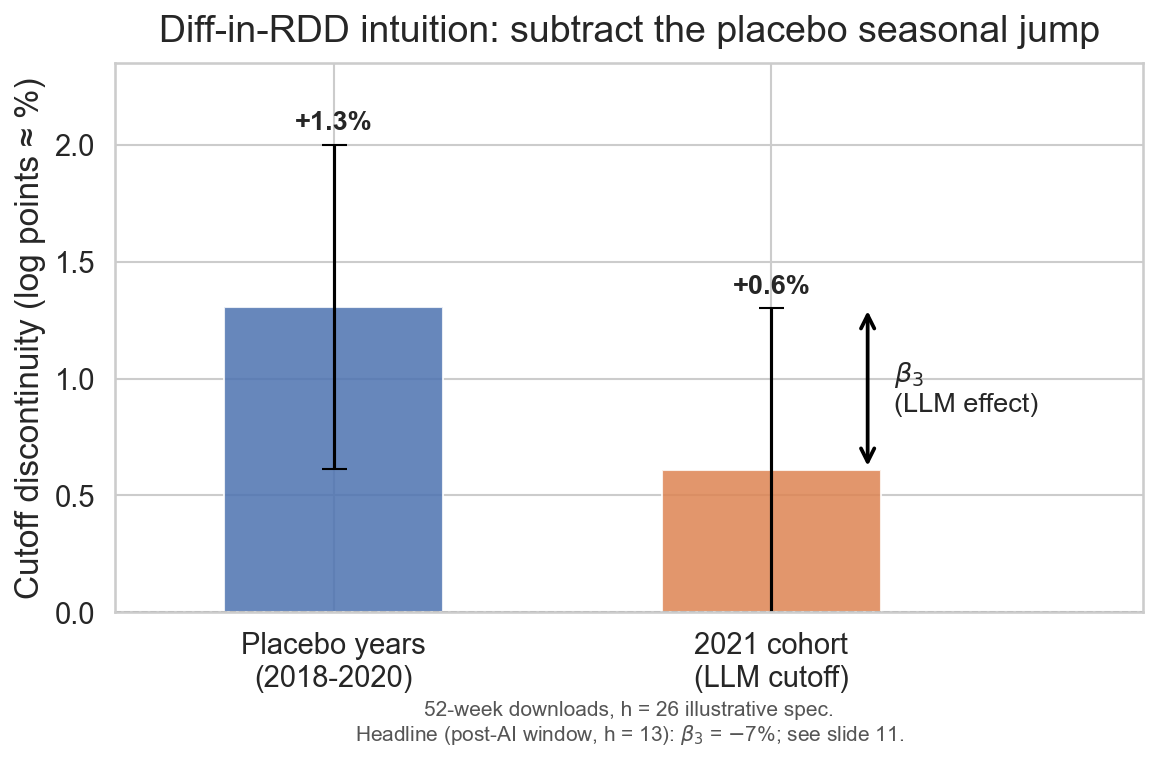
\includegraphics[width=\linewidth]{stacked_rdd_comparison.png}\\
            \footnotesize 2018--2020 placebo coefficients vs.\ 2021. Only 2021 is significant.
        \end{column}
    \end{columns}
\end{frame}

\begin{frame}{A5. GitHub mechanism results}
    \centering
    \footnotesize
    \begin{tabular}{llrrr}
        \toprule
        Tier & Outcome & Excess jump & SE & $p$ \\
        \midrule
        Broad      & All-time imports     & $+2.12$ & 0.92 & \textbf{0.022} \\
        Broad      & Post-AI imports      & $+1.87$ & 1.05 & 0.075 \\
        Successful & All-time imports     & $+2.29$ & 0.96 & \textbf{0.017} \\
        Successful & Post-AI imports      & $+2.09$ & 1.15 & 0.069 \\
        \bottomrule
    \end{tabular}
    \vspace{0.8em}
    \begin{itemize}
        \footnotesize
        \item Baseline-adjusted Diff-in-RDD on log(1 + GitHub imports), $N = 6{,}582$ (Broad).
        \item Positive sign: post-cutoff libraries accumulate \emph{more} imports --- consistent with stock-vs-flow interpretation.
    \end{itemize}
\end{frame}

\begin{frame}{A6. Reviewer comments placeholder}
    \begin{block}{Notes for discussion}
        \begin{itemize}
            \item \textit{[to be populated during Q\&A]}
            \item
            \item
            \item
        \end{itemize}
    \end{block}
\end{frame}

\end{document}
